% Conceptual vector diagrams inspired by the communication-pattern analysis in
% Dimitrov and Skjellum (2001), Figures 7 and 8.
%
% The original figures report message counts and sizes in tabular form. These
% sequence diagrams are an explanatory adaptation, not a reproduction of an
% original message trace.
%
% The generated PDF contains two independently cropped pages:
%   page 1 -- point-to-point send/recv and collective allreduce patterns;
%   page 2 -- synchronous regional dependency chains verified in RDG.
\documentclass[tikz,border=8pt,multi=tikzpicture]{standalone}

\usepackage[T1]{fontenc}
\usepackage{lmodern}
\usepackage{amsmath}
\usetikzlibrary{arrows.meta,backgrounds,fit,positioning}

\definecolor{DimBlue}{HTML}{286FA3}
\definecolor{DimBlueFill}{HTML}{E6F2FA}
\definecolor{DimOrange}{HTML}{D97721}
\definecolor{DimOrangeFill}{HTML}{FFF1DF}
\definecolor{DimGreen}{HTML}{39865B}
\definecolor{DimGreenFill}{HTML}{E8F5EC}
\definecolor{DimPurple}{HTML}{7353A6}
\definecolor{DimPurpleFill}{HTML}{F1ECF8}
\definecolor{DimRed}{HTML}{A61E1E}
\definecolor{DimInk}{HTML}{20242A}
\definecolor{DimMuted}{HTML}{626A73}
\definecolor{DimRule}{HTML}{B9C0C8}

\begin{document}

% Page 1: abstract communication patterns.
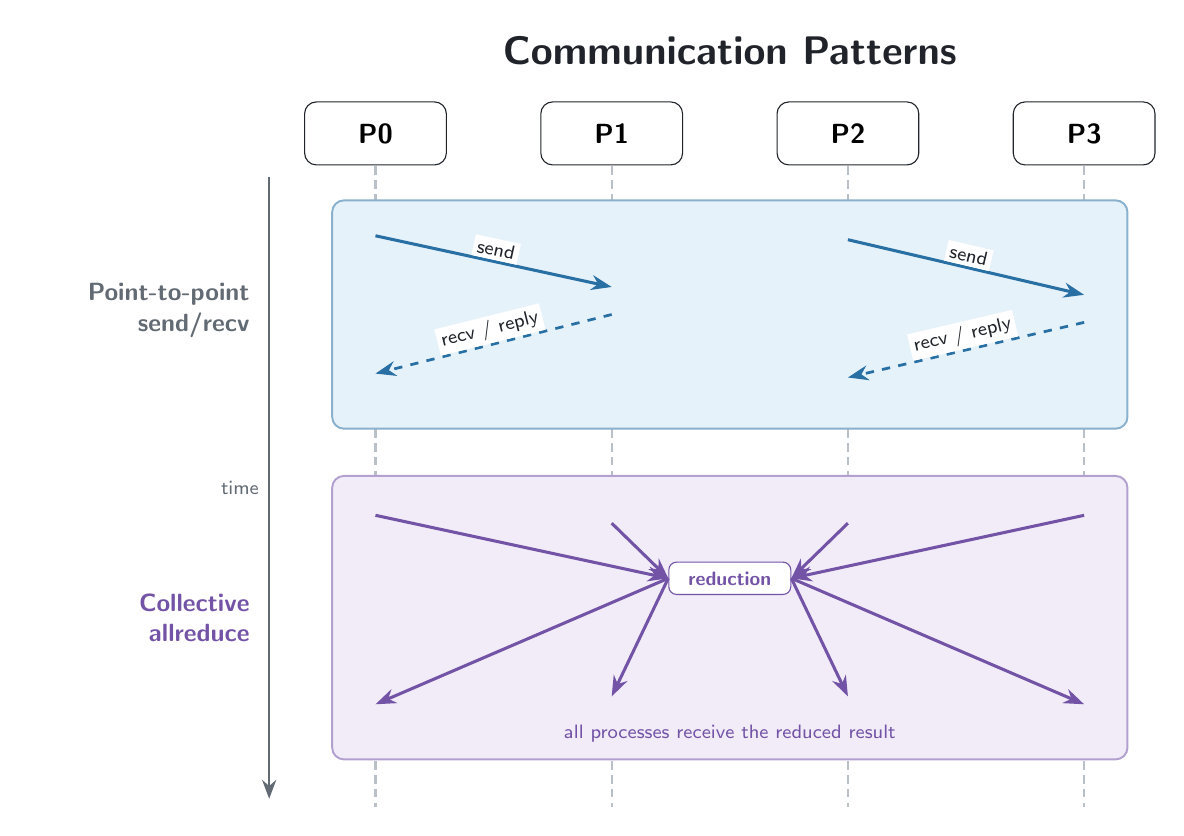
\begin{tikzpicture}[
    font=\sffamily,
    process/.style={
        draw=DimInk,
        rounded corners=1.5mm,
        fill=white,
        minimum width=18mm,
        minimum height=8mm,
        font=\sffamily\bfseries
    },
    lifeline/.style={draw=DimRule, densely dashed, line width=0.8pt},
    message/.style={-{Stealth[length=2.6mm,width=1.9mm]},
                    draw=DimBlue, line width=1.1pt},
    reply/.style={-{Stealth[length=2.6mm,width=1.9mm]},
                  draw=DimBlue, line width=1.0pt, dashed},
    collective/.style={-{Stealth[length=2.6mm,width=1.9mm]},
                       draw=DimPurple, line width=1.1pt},
    msg label/.style={fill=white, inner sep=1.4pt,
                     font=\sffamily\scriptsize, text=DimInk},
    phase label/.style={align=right, text width=27mm,
                       font=\sffamily\small\bfseries, text=DimMuted}
]
    \node[font=\sffamily\bfseries\Large, text=DimInk] at (4.5,1.05)
        {Communication Patterns};

    \foreach \x/\name in {0/P0,3/P1,6/P2,9/P3} {
        \node[process] (\name) at (\x,0) {\name};
        \draw[lifeline] (\x,-0.42) -- (\x,-8.55);
    }

    \draw[-{Stealth[length=2.4mm]}, draw=DimMuted, line width=0.8pt]
        (-1.35,-0.55) -- node[left, font=\sffamily\scriptsize, text=DimMuted]
        {time} (-1.35,-8.45);

    \node[phase label] at (-2.95,-2.25) {Point-to-point\\send/recv};
    \filldraw[fill=DimBlueFill, draw=DimBlue!55, rounded corners=1.5mm,
              line width=0.7pt]
        (-0.55,-0.85) rectangle (9.55,-3.75);

    \draw[message] (0,-1.30) -- node[msg label, above, sloped]
        {send} (3,-1.95);
    \draw[reply] (3,-2.30) -- node[msg label, above, sloped]
        {recv / reply} (0,-3.05);
    \draw[message] (6,-1.35) -- node[msg label, above, sloped]
        {send} (9,-2.05);
    \draw[reply] (9,-2.40) -- node[msg label, above, sloped]
        {recv / reply} (6,-3.10);

    \node[phase label, text=DimPurple] at (-2.95,-6.15)
        {Collective\\allreduce};
    \filldraw[fill=DimPurpleFill, draw=DimPurple!55, rounded corners=1.5mm,
              line width=0.7pt]
        (-0.55,-4.35) rectangle (9.55,-7.95);

    \node[draw=DimPurple, fill=white, rounded corners=1mm,
          font=\sffamily\scriptsize\bfseries, text=DimPurple,
          inner xsep=2.5mm, inner ysep=1.2mm] (reduce) at (4.5,-5.65)
        {reduction};

    \draw[collective] (0,-4.85) -- (reduce.west);
    \draw[collective] (3,-4.95) -- (reduce.west);
    \draw[collective] (6,-4.95) -- (reduce.east);
    \draw[collective] (9,-4.85) -- (reduce.east);

    \draw[collective] (reduce.west) -- (0,-7.25);
    \draw[collective] (reduce.west) -- (3,-7.15);
    \draw[collective] (reduce.east) -- (6,-7.15);
    \draw[collective] (reduce.east) -- (9,-7.25);

    \node[font=\sffamily\scriptsize, text=DimPurple, fill=DimPurpleFill,
          inner sep=1.2pt] at (4.5,-7.62)
        {all processes receive the reduced result};
\end{tikzpicture}

% Page 2: regional synchronous dependencies.
% The context and FHIR paths remain separate because the verified RDG model
% does not use RVE-130 as a FHIR transaction.
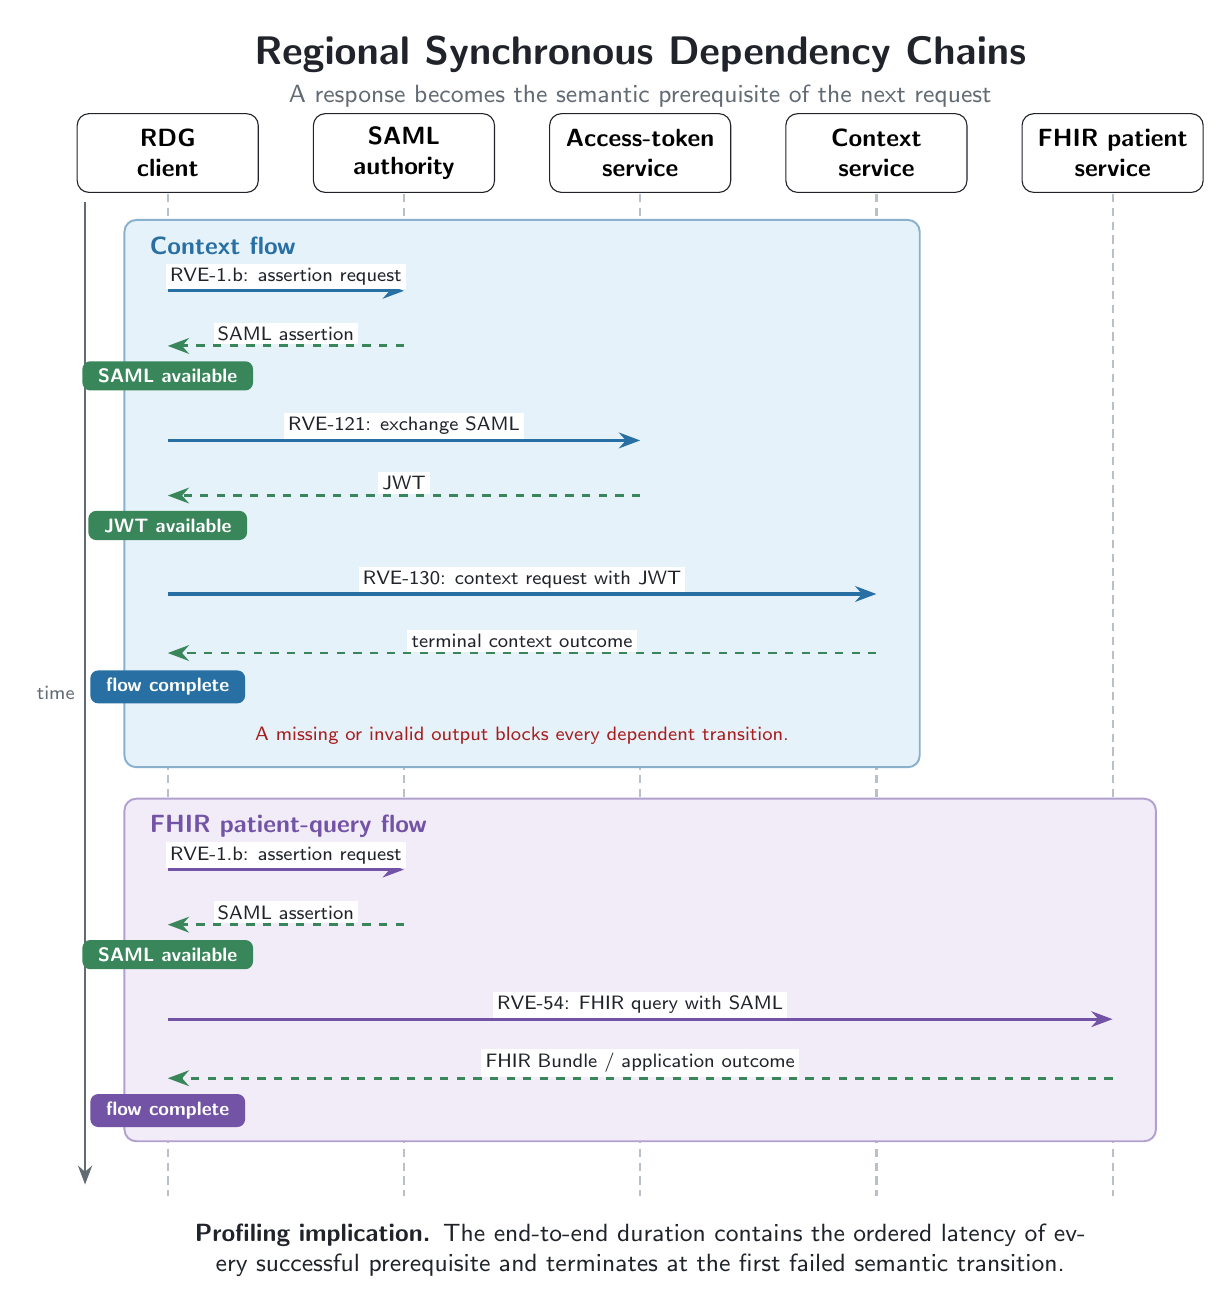
\begin{tikzpicture}[
    font=\sffamily,
    actor/.style={
        draw=DimInk,
        rounded corners=1.5mm,
        fill=white,
        minimum width=23mm,
        minimum height=10mm,
        align=center,
        font=\sffamily\small\bfseries
    },
    lifeline/.style={draw=DimRule, densely dashed, line width=0.8pt},
    call/.style={-{Stealth[length=2.7mm,width=2.0mm]},
                 draw=DimBlue, line width=1.15pt},
    result/.style={-{Stealth[length=2.7mm,width=2.0mm]},
                   draw=DimGreen, line width=1.05pt, dashed},
    fhir call/.style={-{Stealth[length=2.7mm,width=2.0mm]},
                      draw=DimPurple, line width=1.15pt},
    message label/.style={fill=white, inner sep=1.5pt,
                         align=center, font=\sffamily\scriptsize,
                         text=DimInk},
    token/.style={rounded corners=1mm, inner xsep=2mm, inner ysep=1mm,
                  font=\sffamily\scriptsize\bfseries, text=white}
]
    \node[font=\sffamily\bfseries\Large, text=DimInk] at (6.0,1.25)
        {Regional Synchronous Dependency Chains};
    \node[font=\sffamily\small, text=DimMuted] at (6.0,0.72)
        {A response becomes the semantic prerequisite of the next request};

    \node[actor] (rdg) at (0,0) {RDG\\client};
    \node[actor] (saml) at (3,0) {SAML\\authority};
    \node[actor] (token) at (6,0) {Access-token\\service};
    \node[actor] (context) at (9,0) {Context\\service};
    \node[actor] (fhir) at (12,0) {FHIR patient\\service};

    \foreach \x in {0,3,6,9,12} {
        \draw[lifeline] (\x,-0.52) -- (\x,-13.25);
    }
    \draw[-{Stealth[length=2.4mm]}, draw=DimMuted, line width=0.8pt]
        (-1.05,-0.62) -- node[left, font=\sffamily\scriptsize, text=DimMuted]
        {time} (-1.05,-13.10);

    % Context-service flow: RVE-1.b -> RVE-121 -> RVE-130.
    \filldraw[fill=DimBlueFill, draw=DimBlue!55, rounded corners=1.5mm,
              line width=0.7pt]
        (-0.55,-0.85) rectangle (9.55,-7.80);
    \node[anchor=west, font=\sffamily\small\bfseries, text=DimBlue]
        at (-0.35,-1.18) {Context flow};

    \draw[call] (0,-1.75) -- node[message label, above]
        {RVE-1.b: assertion request} (3,-1.75);
    \draw[result] (3,-2.45) -- node[message label, above]
        {SAML assertion} (0,-2.45);
    \node[token, fill=DimGreen] at (0,-2.83) {SAML available};

    \draw[call] (0,-3.65) -- node[message label, above]
        {RVE-121: exchange SAML} (6,-3.65);
    \draw[result] (6,-4.35) -- node[message label, above]
        {JWT} (0,-4.35);
    \node[token, fill=DimGreen] at (0,-4.73) {JWT available};

    \draw[call] (0,-5.60) -- node[message label, above]
        {RVE-130: context request with JWT} (9,-5.60);
    \draw[result] (9,-6.35) -- node[message label, above]
        {terminal context outcome} (0,-6.35);
    \node[token, fill=DimBlue] at (0,-6.78) {flow complete};

    \node[font=\sffamily\scriptsize, text=DimRed, align=center]
        at (4.5,-7.40)
        {A missing or invalid output blocks every dependent transition.};

    % FHIR patient-query flow: RVE-1.b -> RVE-54.
    \filldraw[fill=DimPurpleFill, draw=DimPurple!55, rounded corners=1.5mm,
              line width=0.7pt]
        (-0.55,-8.20) rectangle (12.55,-12.55);
    \node[anchor=west, font=\sffamily\small\bfseries, text=DimPurple]
        at (-0.35,-8.55) {FHIR patient-query flow};

    \draw[fhir call] (0,-9.10) -- node[message label, above]
        {RVE-1.b: assertion request} (3,-9.10);
    \draw[result] (3,-9.80) -- node[message label, above]
        {SAML assertion} (0,-9.80);
    \node[token, fill=DimGreen] at (0,-10.18) {SAML available};

    \draw[fhir call] (0,-11.00) -- node[message label, above]
        {RVE-54: FHIR query with SAML} (12,-11.00);
    \draw[result] (12,-11.75) -- node[message label, above]
        {FHIR Bundle / application outcome} (0,-11.75);
    \node[token, fill=DimPurple] at (0,-12.16) {flow complete};

    \node[anchor=north, align=center, text width=13.2cm,
          font=\sffamily\small, text=DimInk] at (6.0,-13.48)
        {\textbf{Profiling implication.} The end-to-end duration contains the
         ordered latency of every successful prerequisite and terminates at the
         first failed semantic transition.};
\end{tikzpicture}

\end{document}
